%% РУССКОЕ ЗЕРКАЛО статьи для AAAI-27 — ДЛЯ ПРОВЕРКИ, НЕ ДЛЯ ПОДАЧИ.
%% Шаблон AAAI (aaai2027) запрещает кириллицу в тексте, поэтому это зеркало собрано
%% на обычном двухколоночном article + babel(russian) + tempora (как в журнальной RU-версии).
%% Содержание зеркалит ../en/main.tex. Не анонимно (зеркало не подаётся в AAAI).
%% Сборка: pdflatex main_ru ; bibtex main_ru ; pdflatex main_ru ; pdflatex main_ru
\documentclass[10pt,twocolumn,letterpaper]{article}

\usepackage[T2A]{fontenc}
\usepackage[utf8]{inputenc}
\usepackage[english,russian]{babel}
\usepackage{tempora}                       % Times-клон с полной кириллицей (жирная/курсив в T2A)
\usepackage[protrusion=true,expansion=false]{microtype}
\usepackage[letterpaper,margin=0.75in]{geometry}
\setlength{\columnsep}{0.3in}
\usepackage{graphicx}
\graphicspath{{../../../shared/figures/}}
\usepackage{amsmath,amssymb}
\usepackage{booktabs}
\usepackage{array}
\usepackage{cite}

\begin{document}
\twocolumn[{%
  \begin{center}
  \LARGE\bfseries Кросс-возрастная верификация лиц\\ по добытым парам одного человека из соцсетей\\[0.5em]
  \large\mdseries Д.~Ф.~Вольхин \quad И.~С.~Копылов\\[0.25em]
  \normalsize НИУ «Высшая школа экономики», Москва, Россия\quad\texttt{deneal123@mail.ru}
  \end{center}
  \vspace{0.6em}
  \begin{center}\small\itshape
  Русское зеркало для проверки. Это \textbf{не} материал для подачи в AAAI: шаблон AAAI
  запрещает кириллицу в тексте, поэтому официальная подача — англоязычная (\texttt{../en/}).
  \end{center}
  \vspace{0.6em}
  {\small\noindent\textbf{Аннотация.}\enspace Кросс-возрастная верификация лиц — определить, изображён ли на
  двух снимках с разницей в годы один человек — сложна, а longitudinal-данные для обучения редки.
  Мы задаём \emph{data-centric}-вопрос: можно ли получить супервизию для возрастной инвариантности
  без вручную размеченного longitudinal-набора? Мы показываем, что мультифото «тогда/сейчас»-посты
  дают слабые пары \emph{одного человека} без ручных меток личности и возраста (LLM разбирает подписи,
  а кластеризация эмбеддингов формирует личности; компоненты мы аудируем, включая небольшую ручную
  валидацию), и что дообучение намеренно слабого распознавателя на них даёт \emph{переносимую,
  целевую} устойчивость на больших возрастных разрывах. На внешнем бенчмарке FG-NET ROC-AUC на
  большом разрыве ($\geq$25 лет) растёт \textbf{с 0.736 до 0.848} ($+$0.112$\pm$0.001 по трём сидам;
  DeLong $p<10^{-19}$) ценой $-$0.019 точности на LFW и \emph{существенной} деградации при низком FAR
  — это целевой выигрыш для поиска, а не апгрейд универсального верификатора. Наше центральное,
  ограниченное утверждение: внутри протокола атрибуции со слабым backbone \emph{источник данных}, а
  не выбор среди проверяемых целевых функций, объясняет бо\'{}льшую часть прироста (контрастив
  совпадает с ArcFace-margin: 0.848 против 0.851). Прирост обеспечивается парностью одного человека
  (явные возрастные «якоря» из подписей дают лишь $+$0.009), механистически связан с устранением
  возрастного shortcut, превосходит реальную модель пере-старения при контроле паритета разрыва и
  переносится на независимую не-VK платформу.\par}
  \vspace{1.2em}
}]

\section{Введение}\label{sec:intro}
Кросс-возрастная верификация лиц возникает в архивном поиске, восстановлении доступа и авторизованном
поиске пропавших людей. Сложность не в различении произвольных людей, а в отделении \emph{одного
человека сквозь возраст} от \emph{разных людей схожего возраста и внешности}. Разметка longitudinal-пар
(один человек через много лет) дорога, и таких данных мало, что ограничивает supervised-подходы;
недавние работы продолжают сообщать о слабой кросс-датасетной обобщаемости и нехватке качественных
longitudinal-данных.

\textbf{Гипотеза.} Мультифото «тогда/сейчас»-пост с одним человеком в разном возрасте даёт
$\binom{n}{2}$ позитивных пар без ручной разметки; подпись с возрастами добавляет вторичный возрастной
«якорь». Парность одного человека — основной сигнал (абляция изолирует возрастной якорь на уровне лишь
$+$0.009); это масштабируемый, слабо/естественно-супервизируемый сигнал кросс-возрастной идентичности,
и дообучение слабого распознавателя на нём должно переноситься на внешние бенчмарки.

\textbf{Вклад (ограниченный).}
(1)~Слабо/естественно-супервизируемый (без ручных меток личности/возраста) longitudinal-сигнал из
соцпостов — пары одного человека, где возрастные якори лишь вторичны.
(2)~Строгий \emph{протокол атрибуции} (один слабый обучаемый backbone, frozen против дообученного,
внешняя оценка), изолирующий вклад \emph{данных} от ёмкости сети.
(3)~Взаимоподкрепляющие контроли (семейство потерь, архитектура, источник-сообщество, целевая функция,
реальное-против-синтетического, диагностика shortcut, кросс-платформенный перенос), поддерживающие
ограниченное утверждение, что внутри протокола и среди проверенных целей данные дают больше прироста на
большом разрыве, чем выбор семейства потерь.
(4)~Конвейер очистки с аудитом автоматических компонентов и находкой, что наивный счёт позитивов
завышен примерно вдвое near-duplicate-кадрами.
Новизна data-centric, а не архитектурная — новый \emph{источник супервизии}. Перенесённые ради места
контроли и аудиты собраны в дополнительном техническом приложении.

\section{Связанные работы и позиционирование}\label{sec:related}
Наиболее релевантны три линии. \emph{Дискриминативная возраст-инвариантная FR на размеченных данных:}
OE-CNN~\cite{wang2018oecnn}, DAL~\cite{wang2019dal}, MTLFace~\cite{huang2021mtlface} достигают высокой
точности, но обучаются на наборах с \emph{ручными метками личности и возраста} (CACD~\cite{chen2014cacd},
MORPH~\cite{ricanek2006morph}, AgeDB~\cite{moschoglou2017agedb}, FG-NET~\cite{panis2016fgnet}).
\emph{Кросс-возрастной контрастив с синтетикой:} CACon~\cite{wang2024cacon} добавляет синтезированный
кросс-возрастной образец и triplet-потерю; OrdCon~\cite{wang2025ordcon} — order-enhanced контрастив.
\emph{Синтетическое старение:} систематические исследования показывают лишь частичную пользу синтетики
\cite{yao2024synthageing}. Обобщённый self-supervised (аугментации в духе SimCLR~\cite{chen2020simclr})
лишён якорей идентичности во времени. Мы же добываем структуру «один пост $=$ один человек в разном
возрасте» как генератор позитивных пар без меток. Мы отчитываемся на канонических кросс-возрастных
бенчмарках (AgeDB-30, CALFW~\cite{zheng2017calfw}, FG-NET; CALFW — более сложный, возрастно-разнесённый
LFW~\cite{huang2007lfw}). Цель — \emph{не} превзойти абсолютный SOTA (мы берём слабый backbone ради
чистой атрибуции), а измерить величину и переносимость прироста от естественно-супервизируемого
источника; разд.~\ref{sec:res-main} обучает каноническую SOTA-цель прямо на наших данных.

\section{Данные: естественно-заякоренные longitudinal-пары}\label{sec:data}
\textbf{Источник.} Два публичных «тогда/сейчас» мультифото-сообщества во ВКонтакте (одна платформа,
русскоязычный контекст). Лица детектируются и выравниваются по 5-точечному шаблону ArcFace (InsightFace
RetinaFace~\cite{deng2020retinaface}, \texttt{buffalo\_l}). \emph{Пригодное} лицо проходит проверки на
det-score, минимальный размер, размытие и единственность цели. Сырой добытый корпус — в табл.~\ref{tab:scale}.

\begin{table*}[t]
\centering
\small
\begin{tabular}{@{}lrrrrr@{}}
\toprule
Этап & Постов & Фото & Пригодных лиц & Личностей (групп) & Позитивных пар \\
\midrule
Сырой майнинг (2 сообщества) & 44{,}609 & 84{,}147 & 49{,}606 & 21{,}848 & 65{,}897 \\
\textbf{После очистки} & --- & --- & \textbf{40{,}586} & \textbf{21{,}427} & \textbf{31{,}865} \\
\bottomrule
\end{tabular}
\caption{Масштаб набора (сырой майнинг) и после очистки. Удаление near-duplicate-кадров примерно
вдвое сокращает число позитивов.}
\label{tab:scale}
\end{table*}

\textbf{Извлечение возраста.} Подписи разбираются регулярными выражениями (русские паттерны плюс формат
со слешами «6/18/21») и большой языковой моделью (LLM). По всем 33{,}697 мультифото-подписям LLM
расширяет и регуляризует извлечение относительно regex (не читает календарные годы или разрывы как
возраст, восстанавливает второй возраст), расходясь на 27.2\% постов преимущественно в пользу LLM; на
ручном эталоне из 100 подписей LLM совпал с человеком в 89\% против 71\% у regex (приложение). Выход LLM
не считается истиной: ниже по конвейеру явные возрастные якори дают лишь маргинальный вклад
(разд.~\ref{sec:res-main}).

\textbf{Личности и сплит без утечек.} Наивное «один пост $=$ одна личность» недосчитывает: человек
повторяется в разных постах. Мы кластеризуем пост-группы в личности по близости эмбеддингов (косинус
$\geq$ 0.85), получая 21{,}848 личностей из 27{,}487 пост-групп ($\approx$20\% повторов), и делим
\emph{по человеку} (не по посту). Ручной осмотр показал, что косинус не отделяет двойников от одного
человека в полосе 0.55--0.8, поэтому порог слияния намеренно консервативен.

\textbf{Аудит супервизии.} Автоматические компоненты — потенциальный скрытый шум меток, проверяемый
тремя способами: согласие LLM и regex по возрасту; внутригрупповая согласованность кажущегося пола как
дешёвый детектор нескольких людей; и \emph{небольшая} ручная валидация (один аннотатор), которая
\emph{проверяет} конвейер на вменяемость (возраст, целостность групп, точность пар и слияний $0.93$--$0.96$;
приложение). С одним аннотатором и без межаннотаторной $\kappa$ это \emph{поддерживает}, но не
\emph{сертифицирует} супервизию; масштабный многоаннотаторный аудит вне наших ресурсов, поэтому
остаточный шум честно отмечен как ограничение (разд.~\ref{sec:limitations}).

\textbf{Очистка и её главная находка.} Мы применяем поличностную агрегацию кажущегося пола/возраста,
LLM-валидацию целостности групп (92.8\% — один человек) и удаление near-duplicate внутри личности
(косинус $\geq$ 0.97). Поскольку число позитивов квадратично по числу лиц в группе, удаление
near-duplicate сократило счёт позитивов с 65{,}897 до 31{,}865 ($-$52\%): \textbf{около половины сырых
«позитивов» были дублирующими кадрами} (одна съёмка, серия, репост), завышавшими внутренние метрики.
После очистки frozen-базлайн на внутреннем тесте падает (our.25+ $0.705\!\rightarrow\!0.640$), обнажая
более трудный и репрезентативный бенчмарк; внешние бенчмарки не затронуты. Сокращение устойчиво к порогу
дедупа $0.93$--$0.97$ (приложение). Поля происхождения, прав и governance хранятся поэлементно; полная
карточка датасета~\cite{gebru2021datasheets} сопровождает релиз (см.\ раздел об этике).

\section{Метод, протокол и статистика}\label{sec:method}
\textbf{Протокол атрибуции.} Сравнивать адаптер поверх \emph{замороженного} сильного ArcFace с frozen
ArcFace некорректно (адаптер лишь деформирует почти идеальные эмбеддинги). Вместо этого мы берём
\emph{один слабый обучаемый backbone} (FaceNet InceptionResnetV1~\cite{schroff2015facenet}, CASIA-WebFace)
и сравниваем (а)~frozen $\rightarrow$ метрика против (б)~мягкого дообучения головы на наших парах
$\rightarrow$ метрика, с margin-контрастивной потерей. \emph{Оценка — на внешних бенчмарках} (LFW,
AgeDB-30, CALFW, FG-NET) ради чистой атрибуции переноса; внутренний тест (\texttt{our.*}) — вторичная
in-domain диагностика. Сила backbone варьируется (разд.~\ref{sec:res-headroom}). Дизайн меняет
абсолютную производительность на \emph{причинную атрибуцию}.

\textbf{Backbone и метрики.} FaceNet (слабый); ArcFace iResNet-50~\cite{deng2019arcface} (слабый, другая
архитектура); AdaFace IR-50/IR-101~\cite{kim2022adaface} и ArcFace iResNet-100 (сильные; чистый контроль
глубины). Сообщаем LFW (точность по 10 фолдам), AgeDB-30 и CALFW (ROC-AUC и точность) и FG-NET (ROC-AUC
в целом и на подмножестве большого разрыва $\geq$25 лет), различая \emph{беспороговые} метрики (ROC-AUC)
и \emph{пороговые} (точность, TAR@FAR).

\textbf{Статистика.} \emph{Основная конечная точка} — ROC-AUC FG-NET на большом разрыве, нулевая
гипотеза: дообучение не улучшает её относительно frozen (прирост $\leq 0$); AgeDB-30, CALFW и внутренний
кросс-возрастной тест вторичны, лёгкая точность LFW — контроль забывания. Headline-прирост — среднее
$\pm$ std по трём сидам. Мы приводим bootstrap-ДИ, EER и TAR@FAR (внутренний тест дополнительно использует
identity-level bootstrap), тест DeLong для двух \emph{коррелированных} ROC-кривых~\cite{delong1988},
парный permutation-тест и поправку Холма по стратифицированным fairness-тестам (полные таблицы
операционных точек — в приложении). Все headline-эксперименты — на очищенных данных (21{,}427 групп,
40{,}586 лиц, 31{,}865 позитивов; сплит по человеку со сбалансированными негативами).

\section{Результаты}\label{sec:results}
\subsection{Главный эффект и абляция источника супервизии}\label{sec:res-main}
Слабый FaceNet, мягко дообученный на наших парах, поднимает ROC-AUC FG-NET на большом разрыве
\textbf{с 0.736 до 0.848} ($+$0.112$\pm$0.001), при этом лёгкая LFW падает лишь на $-$0.019, а
AgeDB-30/CALFW почти не меняются (табл.~\ref{tab:main}). Абляция изолирует источник: пары из одного
поста не используют ручных меток и дают почти весь прирост; добавление явных возрастных якорей даёт лишь
\textbf{$+$0.009} на бакете 25+. Метод, таким образом, \emph{слабо супервизируется естественной
со-встречаемостью в одном посте}, а возрастная супервизия маргинальна.

\begin{table*}[t]
\centering
\small
\begin{tabular}{@{}lcccc@{}}
\toprule
Метрика & Frozen & $+$pairs (среднее $\pm$ std) & Прирост & (До очистки) \\
\midrule
FG-NET большой разрыв & 0.7361 & 0.8484 $\pm$ 0.0007 & \textbf{$+$0.1124} & $+$0.1215 \\
FG-NET ROC & 0.8955 & 0.9230 $\pm$ 0.0006 & $+$0.0275 & $+$0.0277 \\
our.25+ (внутр.) & 0.6403 & 0.8348 $\pm$ 0.0027 & \textbf{$+$0.1946} & $+$0.1677 \\
our.overall (внутр.) & 0.8363 & 0.9163 $\pm$ 0.0009 & $+$0.0801 & $+$0.0764 \\
LFW точность & 0.9688 & 0.9503 $\pm$ 0.0031 & $-$0.0185 & $-$0.0283 \\
AgeDB-30 ROC & 0.9530 & 0.9462 $\pm$ 0.0013 & $-$0.0068 & $-$0.0155 \\
CALFW ROC & 0.9482 & 0.9489 $\pm$ 0.0014 & $+$0.0007 & $-$0.0030 \\
\bottomrule
\end{tabular}
\caption{Главный результат: слабый FaceNet frozen против $+$pairs, три сида, очищенные данные (прирост
до очистки — для справки). Эффект сосредоточен на подмножестве FG-NET с большим разрывом.}
\label{tab:main}
\end{table*}

Bootstrap-ДИ (сид 42) подтверждают основную точку: FG-NET большой разрыв растёт с 0.736~[0.70, 0.78] до
0.848~[0.82, 0.88] с \emph{непересекающимися} 95\% ДИ; EER почти вдвое снижается (0.335$\to$0.219), а
TAR@FAR$=$1\% почти удваивается (0.21$\to$0.39). Поскольку пересечение bootstrap-ДИ игнорирует общие
образцы двух моделей, мы подтверждаем точку тестом DeLong для коррелированных ROC~\cite{delong1988}: на
FG-NET большом разрыве $z=9.3$, $p=1.4\times10^{-20}$ ($\Delta$AUC 95\% ДИ $[+0.088,+0.135]$); парный
permutation-тест ($10^4$) согласуется ($p<10^{-4}$). Тот же тест показывает целевой характер: AgeDB-30
слегка снижается ($-$0.008, $p=4\times10^{-6}$), а CALFW неизменна ($p=0.95$). Операционные точки
(табл.~\ref{tab:stats}) делают компромисс наглядным: AUC и TAR@1\% на большом разрыве резко растут, а
точки низкого FAR на лёгких бенчмарках (LFW TAR@0.1\%) деградируют.

\begin{table*}[t]
\centering
\small
\begin{tabular}{@{}lccccc@{}}
\toprule
Бенчмарк & Frozen AUC [95\% ДИ] & $+$pairs AUC [95\% ДИ] & EER (fr.$\to$$+$p.) & TAR@1\% & TAR@0.1\% \\
\midrule
FG-NET большой разрыв & 0.736 [0.70, 0.78] & \textbf{0.848 [0.82, 0.88]} & 0.335$\to$0.219 & 0.209$\to$0.386 & 0.074$\to$0.154 \\
FG-NET в целом & 0.896 [0.89, 0.90] & 0.922 [0.92, 0.93] & 0.186$\to$0.151 & 0.502$\to$0.562 & 0.315$\to$0.308 \\
AgeDB-30 & 0.953 [0.95, 0.96] & 0.945 [0.94, 0.95] & 0.115$\to$0.126 & 0.525$\to$0.510 & 0.285$\to$0.309 \\
CALFW & 0.948 [0.94, 0.95] & 0.948 [0.94, 0.95] & 0.116$\to$0.117 & 0.580$\to$0.624 & 0.213$\to$0.320 \\
LFW (AUC) & 0.994 [0.99, 1.00] & 0.987 [0.98, 0.99] & 0.032$\to$0.052 & 0.940$\to$0.869 & 0.858$\to$0.575 \\
\bottomrule
\end{tabular}
\caption{Операционные точки и 95\% bootstrap-ДИ (FaceNet frozen против $+$pairs, сид 42). LFW показан как
ROC-AUC для единообразия.}
\label{tab:stats}
\end{table*}

\textbf{Инвариантность к целевой функции.} Обучая канонические современные margin-цели — ArcFace,
CosFace и SphereFace~\cite{deng2019arcface} (ядро OE-CNN/MTLFace) — на наших естественно-супервизируемых
личностях при том же backbone и протоколе, контрастив, ArcFace и CosFace \textbf{совпадают} на основной
точке (0.848 / 0.851 / 0.843, в пределах $\pm$0.006); лишь SphereFace, труднее всего оптимизируемый на
2--3-shot личностях без $\lambda$-annealing, отстаёт (0.801). Шумоустойчивый sub-center
ArcFace~\cite{deng2020subcenter} также даёт 0.851 — явная машинерия для шума меток ничего не добавляет на
\emph{очищенных} парах. Отсюда ограниченный вывод: внутри протокола и среди проверенных целей
\emph{источник данных} объясняет больше прироста, чем выбор цели (полная таблица — в приложении,
табл.~\ref{tab:objective}).

\begin{table}[t]
\centering
\setlength{\tabcolsep}{3pt}
\small
\begin{tabular}{@{}lcccc@{}}
\toprule
Цель & FG-NET 25+ & our.25+ & LFW & AgeDB-30 \\
\midrule
Frozen & 0.736 & 0.640 & 0.969 & 0.953 \\
$+$pairs (контр.) & 0.848 & 0.838 & 0.946 & 0.945 \\
$+$ArcFace & \textbf{0.851} & 0.868 & 0.952 & 0.947 \\
$+$ArcFace, sub-center & 0.851 & 0.869 & 0.951 & 0.947 \\
$+$CosFace & 0.843 & 0.860 & 0.952 & 0.945 \\
$+$SphereFace & 0.801 & 0.699 & 0.950 & 0.943 \\
\bottomrule
\end{tabular}
\caption{Сравнение целей (FaceNet, очищенные): контрастив, ArcFace и CosFace совпадают на основной
точке; sub-center ничего не добавляет; SphereFace отстаёт на разреженных few-shot личностях.}
\label{tab:objective}
\end{table}

\subsection{Реальные пары превосходят синтетическое старение}\label{sec:res-synth}
Замена реальных позитивов синтетически состаренными — доменным прокси и реальной сетью пере-старения
(FRAN~\cite{zoss2022fran}) — уступает реальным парам, а на дефолтном \emph{широком} разрыве FRAN даже
\emph{падает} ниже frozen (FG-NET большой разрыв 0.727; табл.~\ref{tab:synth}). Идентичность-сохраняющее
старение воспроизводит текстурные артефакты, а не реальную longitudinal-вариативность (поза, камера,
эпоха). Контроль на нативном разрешении исключает артефакт кропа: перекадрирование подмножества на
512\,px прямо из исходников и повторное старение не меняет результат (0.771 против 0.778). Контроль
паритета разрыва уточняет картину: FRAN стареет на широкий разрыв 33--70 лет, тогда как у реальных пар
медиана 9 лет; согласование синтетического разрыва с реальным распределением поднимает FRAN до
\textbf{0.759} — скромный плюс, согласующийся с сообщаемыми приростами синтетики~\cite{yao2024synthageing}
— но реальные пары (0.848) всё равно ведут на $+$0.089. Реальные добытые пары обходят даже
\emph{согласованную по разрыву} модель пере-старения.

\begin{table}[t]
\centering
\setlength{\tabcolsep}{4pt}
\small
\begin{tabular}{@{}lcccc@{}}
\toprule
Метрика & Frozen & $+$реал. & syn-FRAN & FRAN-gm \\
\midrule
FG-NET 25+ & 0.736 & \textbf{0.848} & 0.727 & 0.759 \\
our.25+ & 0.640 & \textbf{0.838} & 0.549 & 0.622 \\
\bottomrule
\end{tabular}
\caption{Реальные против синтетических позитивов (FaceNet, очищенные). FRAN-gm согласует синтетический
возрастной разрыв с распределением реальных пар (медиана 9 лет).}
\label{tab:synth}
\end{table}

\subsection{Headroom и масштабирование по данным}\label{sec:res-headroom}
Прирост воспроизводится на FaceNet, ArcFace iResNet и AdaFace IR-50/IR-101 (три семейства потерь, две
архитектуры) и \emph{монотонно убывает с силой frozen} (рис.~\ref{fig:headroom}); чистый контроль глубины
(AdaFace IR-50 $\rightarrow$ IR-101) это подтверждает. Сильные насыщенные backbone не улучшаются и слегка
забывают при дообучении; мягкая скорость обучения вдвое снижает забывание, но не превращает его в
прирост. Вклад, таким образом, специфичен для слабых и средних backbone с кросс-возрастным запасом — это
ограничение мы прямо отмечаем (разд.~\ref{sec:limitations}). При варьировании доли обучающих личностей
(val/test фиксированы) прирост насыщается рано: \textbf{$\approx$96\% полного прироста FG-NET большого
разрыва достигается уже на 10\% личностей} ($\approx$1{,}500), выходя на плато с 25\%
(рис.~\ref{fig:scaling}; каждая точка — среднее $\pm$ std по трём сидам). Сигнал данных-эффективен;
дальнейший рост требует \emph{более трудных} данных (большие разрывы, трудные позитивы), а не просто
объёма.

\begin{figure}[t]
\centering

\includegraphics[width=\columnwidth]{fig_headroom_ru.pdf}
\caption{Кривая headroom: прирост $+$pairs на FG-NET большом разрыве монотонно сжимается с усилением
frozen-backbone, пересекая ноль для сильных насыщенных моделей.}
\label{fig:headroom}
\end{figure}

\begin{figure}[t]
\centering

\includegraphics[width=\columnwidth]{fig_scaling_ru.pdf}
\caption{Закон масштабирования: внешний (FG-NET большой разрыв) и внутренний (our.25+) ROC-AUC против
числа обучающих личностей (лог-шкала). Около 96\% прироста достигается на 10\% личностей; полосы — $\pm$1
std по трём сидам, пунктир — frozen-базлайны.}
\label{fig:scaling}
\end{figure}

\subsection{Механизм: возрастной shortcut}\label{sec:res-shortcut}
При age-matched негативах (тот же возрастной бакет, разные люди) точность frozen на внутреннем тесте 25+
падает с 0.640 до 0.517 (\textbf{около уровня случайности 0.5}), а реальные пары восстанавливают её до
\textbf{0.838} (рис.~\ref{fig:shortcut}) — прямое свидетельство, что frozen-модели различают
кросс-возрастные пары в основном по \emph{возрасту}, тогда как наши пары наводят различение по
\emph{идентичности}. Линейный проб уточняет это репрезентационно: кажущийся возраст остаётся хорошо
декодируемым из эмбеддинга идентичности у \emph{всех} моделей ($\approx$0.63--0.65 сбалансированной
точности $\gg$ 0.25 случайности) и меняется слабо, тогда как AUC идентичности резко растёт
(0.836$\rightarrow$0.916) — метод учит инвариантную \emph{метрику} (косинус перестаёт опираться на ось
возраста), а не возраст-свободное представление; явное adversarial-разделение не снижает утечку дальше
(приложение).

\begin{figure}[t]
\centering

\includegraphics[width=0.86\columnwidth]{fig_shortcut_ru.pdf}
\caption{Возрастной shortcut: на тесте только-по-идентичности (age-matched негативы) frozen-модель падает
почти до случайности; дообучение на наших парах восстанавливает различение по идентичности.}
\label{fig:shortcut}
\end{figure}

\subsection{Кросс-платформенный и кросс-исходный перенос}\label{sec:res-cross}
Обучение на одном VK-сообществе и тест на отложенном другом переносит прирост (внешний FG-NET большой
разрыв $+$0.113, практически как внутри-исходный $+$0.112). Более сильная внешняя проверка — обобщается ли
\emph{источник} за пределы платформы. Применяя \emph{идентичный} протокол майнинга к независимому не-VK
сообществу — доске Reddit r/PastAndPresentPics (тот же формат «тогда/сейчас», тот же LLM-парсер) — и
оценивая VK-обученную $+$pairs-модель \emph{без} Reddit-данных в обучении на 1{,}575 Reddit-парах, общий
ROC-AUC растёт \textbf{с 0.718 до 0.749} ($+$0.031, почти непересекающиеся 95\% ДИ). Перенос
\emph{двунаправлен}: backbone, обученный \emph{только} на малом 220-личностном Reddit-источнике (пилот, не
headline), тоже помогает на VK (FG-NET большой разрыв $+$0.047). Прирост меньше, чем внутри VK (более
шумный, частично коллажный набор), поэтому мы читаем его как подтверждение обобщения источника за
платформу, а не SOTA-заявку. Рис.~\ref{fig:external} показывает, что прирост $+$pairs остаётся
\emph{положительным на всех трёх} внешних оценках, сжимаясь на более трудных/шумных наборах.

\begin{figure}[t]
\centering
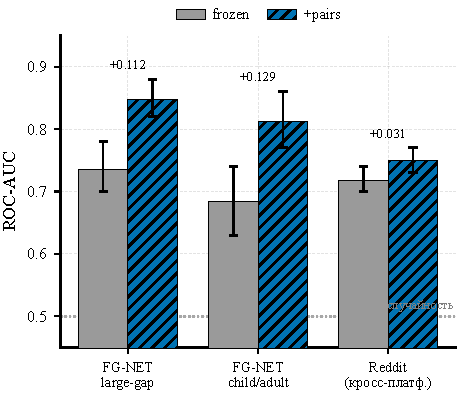
\includegraphics[width=\columnwidth]{fig_external_ru.pdf}
\caption{Внешнее обобщение. Прирост $+$pairs над frozen (95\% ДИ) держится на трёх независимых оценках —
FG-NET большой разрыв, child$\leftrightarrow$adult подмножество FG-NET и кросс-платформенный Reddit —
везде выше случайности, наибольший на in-protocol FG-NET и меньший (но положительный) на более шумном
Reddit.}
\label{fig:external}
\end{figure}

\textbf{Аудит по кажущимся демографиям.} При стратификации по \emph{кажущемуся} полу/возрасту якоря пары
(оценочному, не самоидентифицированному) ни одна группа не деградирует, и каждый прирост значим (95\%
парный bootstrap-ДИ $>$ 0; приложение). Наибольший прирост — у младшей группы 0--17 (0.750$\rightarrow$0.880,
$+$0.130), где базовая модель слабее всего, что подтверждается на \emph{независимом}
child$\leftrightarrow$adult подмножестве FG-NET ($+$0.129, непересекающиеся ДИ). При согласованном
$\approx$1\% FMR $+$pairs снижает FNMR в каждой кажущейся страте. Мы избегаем слова «справедливо» как
решённого свойства: источник смещён к кажущемуся женскому полу (76.7\%), а атрибуты кажущиеся, не
юридические категории.

\section{Обсуждение}\label{sec:discussion}
Вклад — масштабируемый, слабо/естественно-супервизируемый источник longitudinal-супервизии, обучающий
переносимой кросс-возрастной устойчивости, которую синтетическое старение не заменяет, а явная
возрастная супервизия не объясняет. Взаимоподкрепляющие контроли (семейство потерь, архитектура,
источник-сообщество, цель, шумоустойчивый margin) сходятся к ограниченному выводу: внутри протокола
\emph{источник данных} объясняет больше прироста на большом разрыве, чем выбор цели. Важно: улучшение —
\emph{целевой} прирост на большом разрыве, а не drop-in апгрейд универсального верификатора: точки
низкого FAR на лёгких бенчмарках деградируют (LFW TAR@FAR$=$0.1\% падает $0.858\rightarrow0.575$), поэтому
развёртывание следует ограничивать режимом большого кросс-возрастного разрыва.

\textbf{Объём утверждений.} \emph{Установлено (внутри протокола атрибуции):} (i)~пары улучшают верификацию
на большом разрыве на FG-NET (основная точка, непересекающиеся 95\% ДИ) и внутреннем тесте 25+;
(ii)~прирост переносится между двумя сообществами, на независимое child$\leftrightarrow$adult
подмножество FG-NET и на не-VK платформу; (iii)~реальные пары \textbf{превосходят синтетическое старение},
включая контроли нативного разрешения и паритета разрыва; (iv)~прирост инвариантен к контрастиву, ArcFace
и CosFace; (v)~механистически связан с \textbf{устранением возрастного shortcut}; (vi)~около половины
сырых позитивов были near-duplicate-кадрами. \emph{Не установлено / вне объёма:} это не равномерный
прирост верификации (точки низкого FAR деградируют); сильные насыщенные backbone не улучшаются; больший
не-VK \emph{обучающий} источник с многосидовыми ДИ — дальнейшая работа; мы не воспроизводим полный
SOTA-конвейер, только общую margin-цель; fairness-аудит использует лишь кажущиеся атрибуты без
многоаннотаторной $\kappa$.

\section{Ограничения}\label{sec:limitations}
\begin{itemize}
\item \textbf{Зависимость от backbone:} прирост сосредоточен в слабых/средних backbone; сильные
насыщенные не улучшаются и слегка забывают.
\item \textbf{Внешняя валидность:} два VK-сообщества, одна платформа, один язык/культурный контекст;
смещение к кажущемуся женскому полу (76.7\%); разреженность при кажущемся возрасте 45+. Перенос показан
между двумя VK-источниками, на стандартные внешние бенчмарки и на небольшой независимый Reddit-тест
«тогда/сейчас»; это не устанавливает платформо-агностичную обобщаемость.
\item \textbf{Только кажущиеся атрибуты} в fairness-аудите (оценочные, не самоидентифицированные пол/
этничность) и без межаннотаторной $\kappa$ (масштабный ручной аудит трудоёмок и вне наших ресурсов).
\item \textbf{Слабо супервизируется, не label-free:} LLM разбирает возраст и валидирует целостность групп,
а кластеризация формирует личности — проверено, но остаётся источником скрытого шума.
\item \textbf{Масштаб и возраст бенчмарков:} стандартный кросс-возрастной набор (AgeDB-30, CALFW, FG-NET)
обеспечивает сопоставимость, но наследует ограниченный масштаб/возраст; больший не-VK longitudinal-набор
остаётся полезной дальнейшей работой.
\end{itemize}

\section*{Этика, правовая основа и data governance}
Это чувствительное биометрическое исследование; governance мы рассматриваем как полноценный компонент.
Разрешённое использование ограничено controlled / consent-based / human-reviewed приложениями (архивы и
семейные фото с очищенными правами, авторизованный гуманитарный поиск, восстановление доступа); система
выдаёт кандидатов для проверки человеком, а не автоматическое решение. Это \emph{только исследовательская}
работа: ничего не развёртывается и \emph{не публикуется публичная биометрическая база}. Запрещено:
массовая идентификация, деанонимизация, слежка и любая обработка данных несовершеннолетних без правовой
основы.

\emph{Этическое одобрение.} Формальный протокол этического комитета по данному исследованию на текущий
момент не оформлялся; учитывая его исключительно исследовательский характер и полное обезличивание,
авторы оформят этическую экспертизу организации или документированное освобождение, если этого потребует
площадка или рецензенты. \emph{Согласие.} Поскольку данные взяты из публичных постов без реальной
возможности связаться с субъектами, индивидуальное информированное согласие не получалось; мы опираемся
на научно-исследовательскую правовую основу с мерами обезличивания ниже и отмечаем, что официальный доступ
к API и добровольная публикация сами по себе не дают права на биометрическую обработку (ср.\ спецкатегория
по GDPR ст.~9~\cite{gdpr2016} и национальное право о согласии на биометрию).

\emph{Обезличивание и доступ.} Мы \emph{не публикуем сырые изображения лиц и сырые посты}. Публичный релиз
ограничен кодом, конфигурациями, псевдонимизированным протоколом бенчмарка и агрегатной статистикой.
Поскольку эмбеддинг лица сам по себе сравнимый \emph{биометрический шаблон}, а солёные хеши не делают его
анонимным, веса и эмбеддинги предоставляются добросовестным исследователям \emph{по запросу} в рамках
краткого соглашения об использовании в исследовательских целях (только research; запрет реидентификации).
Обезличенный набор данных также доступен по запросу, формальная документация по защите данных будет
подготовлена при необходимости. Идентификаторы платформы заменяются солёными хешами; подписи/комментарии
исключаются; хранятся только возрастной бакет и псевдонимный ID; элементы детского возраста исключаются из
релиза без явных правовых рамок и согласия законного представителя. DPIA, полную карточку
датасета~\cite{gebru2021datasheets} и процедуру удаления по запросу мы прилагаем к релизу.

\textbf{Воспроизводимость.} Мы публикуем все скрипты, конфигурации и версионированные LLM-промпты; сырые
изображения и посты не публикуются, поэтому воспроизведение майнинга частично (мы публикуем кэшированные
выходы LLM для детерминированного replay). Всё исследование выполняется на одном ноутбуке (одна GPU на
6\,ГБ). Чек-лист воспроизводимости прилагается.

\bibliographystyle{IEEEtran}
\bibliography{../../../shared/refs}

\end{document}
